\chapter{Analiza danych}
\label{ch:analiza}

W niniejszym rozdziale przedstawiono wyniki modelowania cen energii za pomocą czterech modeli: regresji liniowej, regresji Ridge, Propheta oraz MLP. Analiza została podzielona na dwa podrozdziały, odpowiadające okresom stabilnemu i niestabilnemu. Zbiór danych został poddany testom w celu oceny skuteczności. W związku z tym dla modeli przeprowadzono strojenie hiperparametrów. 

\section{Okres stabilny}
\label{sec:okres_stabilny}

\subsubsection{Regresja liniowa i Ridge}

Przeanalizowano modele regresji liniowej oraz regresji Ridge na danych z okresu stabilnego. Modele trenowano na danych z lat 2016--2018, a testowano na danych z 2019 roku.

Wyniki dla pełnego zbioru o 60 parametrach wejściowych przedstawiono w tabeli~\ref{tab:linear_ridge_results_full}. Regresja Ridge osiągnęła lepsze wyniki niż regresja liniowa, co jest widoczne w tabeli poniżej na podstawie przedstawionych wcześniej metryk ~\ref{sec:ocena_jakosci_prognoz}. Wynika to z powodu regularyzacji L2 zastosowanej w modelu Ridge. 

\begin{table}[H]
    \centering
    \caption{Wyniki regresji liniowej i grzebietowej dla pełnego zbioru danych w okresie stabilnym (2019).}
    \label{tab:linear_ridge_results_full}
    \begin{tabular}{|l|ccccc|}
        \hline
        \textbf{Model} & \textbf{MAE} & \textbf{RMSE} & \textbf{MAPE (\%)} & \textbf{sMAPE (\%)} & \textbf{\(R^2\)} \\
        \hline
        Regresja liniowa & 15.18 & 19.79 & 7.25 & 7.16 & 0.8413 \\
        Regresja Ridge   & 15.09 & 19.64 & 7.19 & 7.09 & 0.8437 \\
        \hline
    \end{tabular}
\end{table}

Najlepsza wartość hiperparametru \(\alpha\) w regresji Ridge wyniosła 500.0. Wysoka wartość \(\alpha = 500.0\) sugeruje, że w pełnym zbiorze danych występuje istotna współliniowość między zmiennymi objaśniającymi. Potwierdza to również analiza macierzy korelacji ~\ref{fig:correlation_plot}.

Następnie przeprowadzono analizę skróconego zbioru danych opisanego w~\ref{sec:shortened_dataset}. Wyniki dla skróconego zbioru danych są przedstawione w tabeli~\ref{tab:linear_ridge_results_short}, wraz z różnicami w metrykach względem pełnego zbioru danych. Różnice w metrykach wskazują, że dodatkowe zmienne w pełnym zbiorze danych wnoszą informację, mimo niższego poziomu korelacji ze zmienną objaśnianą. Różnice metryk nie są bardzo duże (np. MAPE różni się o 0.16\% dla regresji Ridge), co może sugerować, że skrócony zbiór danych nadal zawiera najważniejsze zmienne objaśniające.

\begin{table}[h]
    \centering
    \caption{Wyniki regresji liniowej i Ridge dla skróconego zbioru danych w okresie stabilnym (2019) wraz z różnicami względem pełnego zbioru.}
    \label{tab:linear_ridge_results_short}
    \begin{tabular}{|l|ccccc|c|}
        \hline
        \textbf{Model} & \textbf{MAE} & \textbf{RMSE} & \textbf{MAPE (\%)} & \textbf{sMAPE (\%)} & \textbf{\(R^2\)} & \textbf{Różnica MAPE (\%)} \\
        \hline
        Regresja liniowa & 15.61 & 20.31 & 7.33 & 7.32 & 0.8328 & +0.08 \\
        Regresja Ridge   & 15.67 & 20.40 & 7.35 & 7.34 & 0.8314 & +0.16 \\
        \hline
    \end{tabular}
\end{table}

W celu potencjalnego polepszenia wyników zastosowano logarytmizację zmiennej wyjściowej (\texttt{fixing\_i\_price}), co miało na celu zmniejszenie skośności rozkładu cen i poprawę dopasowania modelu. Wyniki z logarytmizacją przedstawiono w tabeli~\ref{tab:linear_ridge_results_log}.

\begin{table}[h]
    \centering
    \caption{Wyniki regresji liniowej i Ridge z logarytmizacją dla okresu stabilnego (2019).}
    \label{tab:linear_ridge_results_log}
    \begin{tabular}{|l|ccccc|}
        \hline
        \textbf{Model i zbiór danych} & \textbf{MAE} & \textbf{RMSE} & \textbf{MAPE (\%)} & \textbf{sMAPE (\%)} & \textbf{\(R^2\)} \\
        \hline
        Regresja liniowa (pełny)   & 21.63 & 28.36 & 9.85 & 9.16 & 0.6736 \\
        Regresja Ridge (pełny)     & 19.99 & 26.06 & 9.21 & 8.65 & 0.7244 \\
        Regresja liniowa (skrócony) & 26.36 & 33.07 & 11.95 & 10.94 & 0.5563 \\
        Regresja Ridge (skrócony)   & 23.29 & 29.38 & 10.69 & 9.89 & 0.6498 \\
        \hline
    \end{tabular}
\end{table}

Logarytmizacja nie przyniosła spodziewanych korzyści i pogorszyła wyniki we wszystkich metrykach. Największe pogorszenie zaobserwowano dla skróconego zbioru danych, gdzie MAPE dla regresji liniowej wzrosło do 11.95\%, a \(R^2\) spadło do 0.5563. Przyczyną jest najprawdopodobniej fakt, że logarytmizacja wprowadziła niepotrzebne nieliniowości, które utrudniły dopasowanie modeli liniowych. Dodatkowo, odwrócenie transformacji logarytmicznej może amplifikować błędy predykcji, co wpłynęło na wzrost RMSE i MAE.

Regresja Ridge w porównaniu do regresji liniowej lepiej przewiduje ceny, co potwierdzają wyniki metryk. Poniżej umieszczam wykres rzeczywistych i przewidywanych wartości dla regresji Ridge w okresie stabilnym. Załączony został przykładowy wykres z pierwszego kwartału 2019 roku, aby lepiej zobrazować prognozy modelu.

\begin{figure}[H]
    \centering
    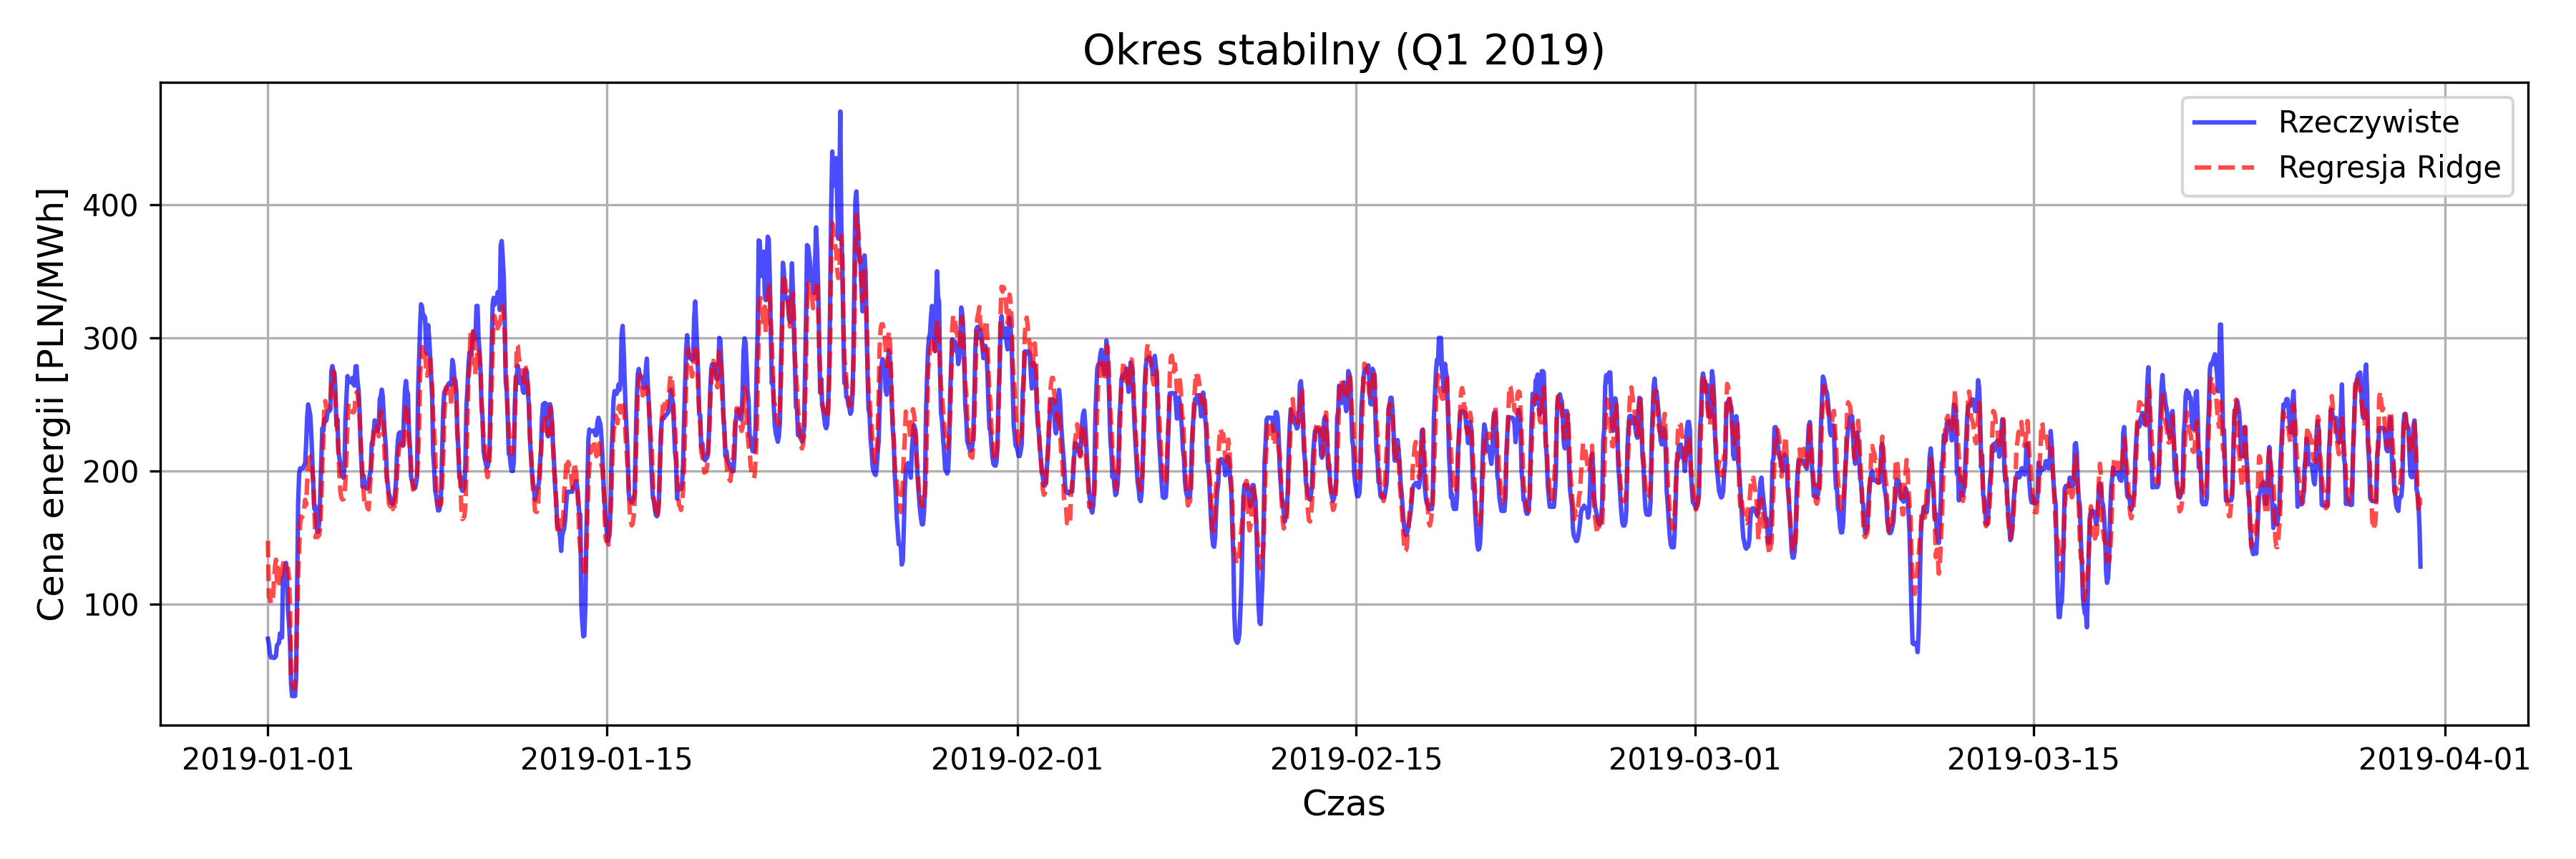
\includegraphics[width=1.0\textwidth]{../../plots/predicts/ridge_predictions_full_q1_2019.png}
    \caption{Porównanie rzeczywistych i przewidywanych wartości cen energii dla regresji Ridge w okresie stabilnym.}
    \label{fig:ridge_predictions_full_stable_period}
\end{figure}

Widoczne na wykresie jest to, że model nie nadążą za dużymi skokami cen energii, prawdopodobnie z powodu ich nieliniowości. Z kolei w przypadku okresów mniejszych zmian i stabilniejszych cen, model oczekuje większej zmienności, co prowadzi do przeszacowania prognoz. Poniżej załączony jest histogram reszt dla regresji Ridge.

\begin{figure}[H]
    \centering
    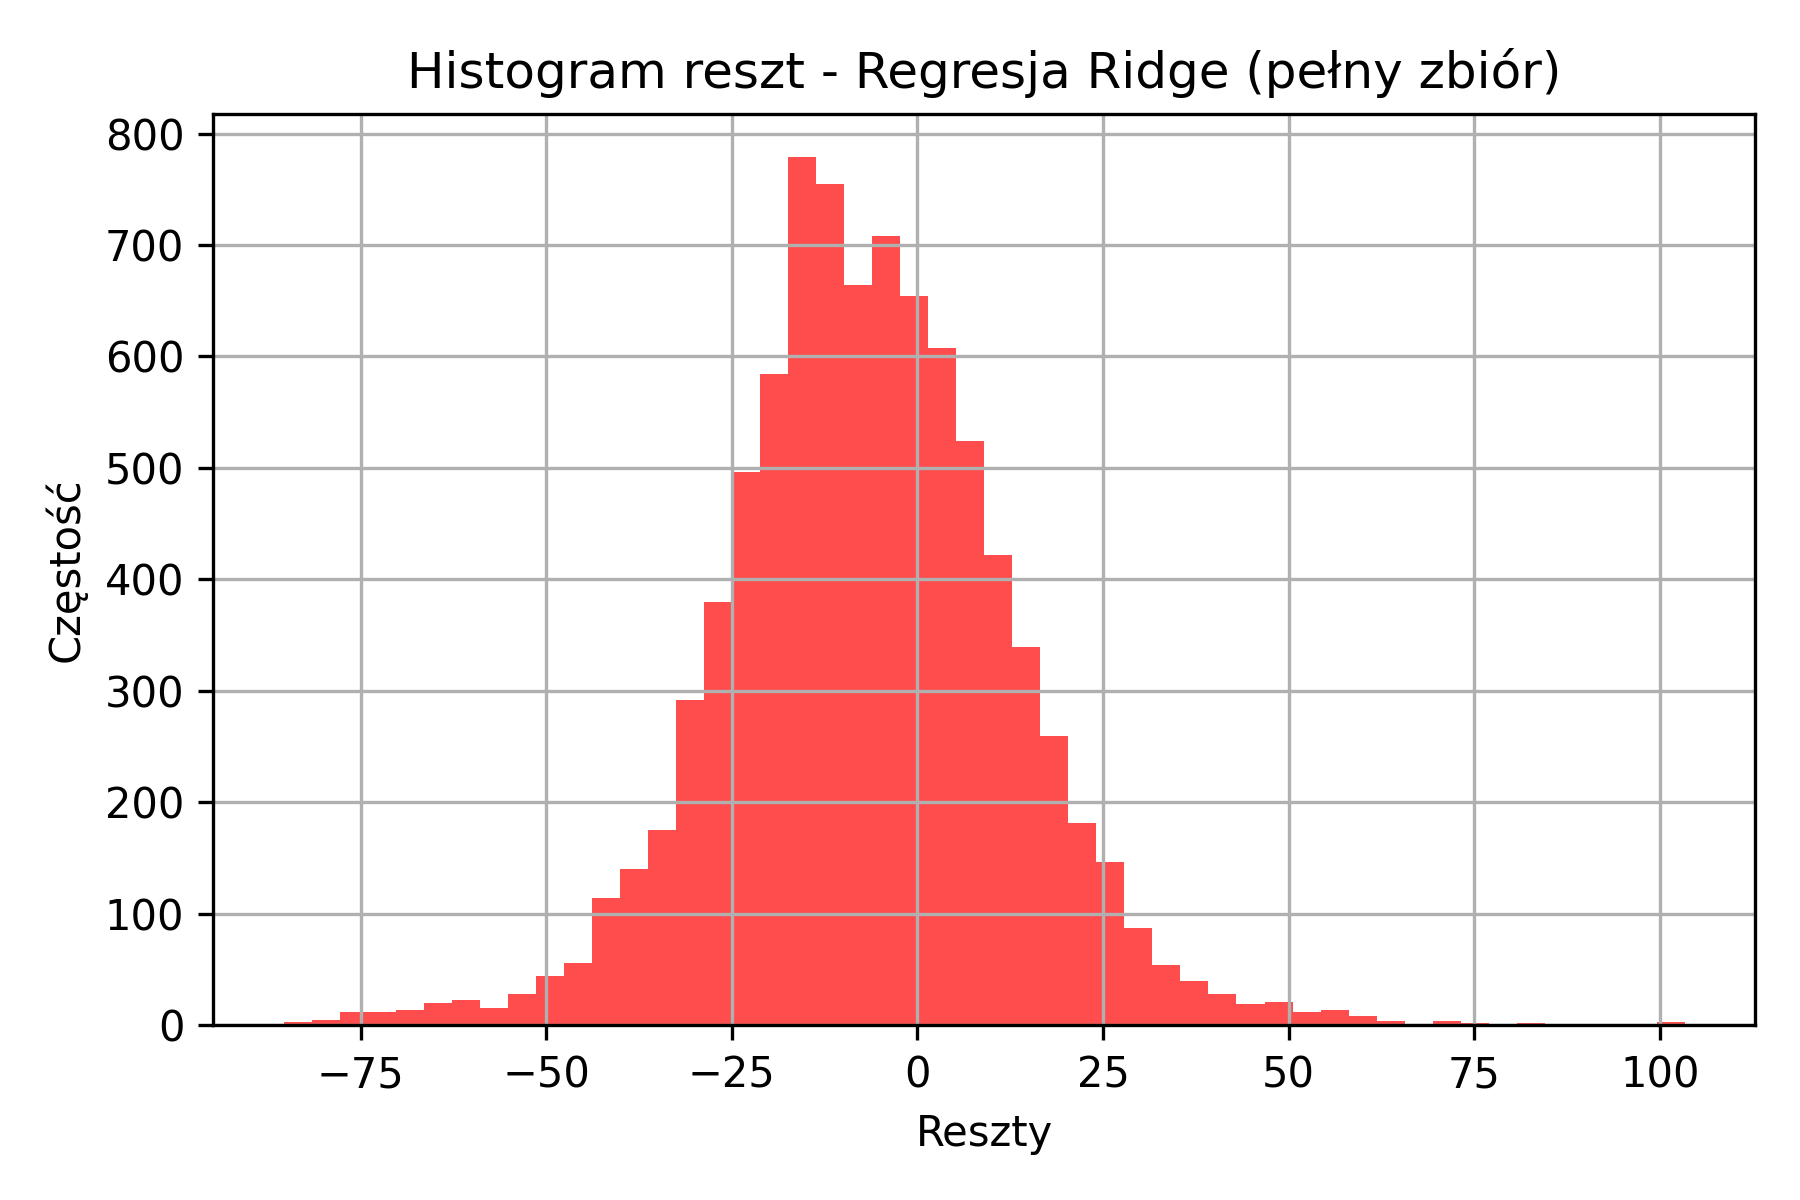
\includegraphics[width=1.0\textwidth]{../../plots/predicts/residuals_histogram_Ridge_full_stable_period.png}
    \caption{Histogram reszt dla regresji Ridge w okresie stabilnym.}
    \label{fig:ridge_residuals_stable_period}
\end{figure}

Histogram posiada szczyt w okolicy zera i większość błędów skupia się w okolicy zera. Rozkład reszt jest zbliżony do normalnego bez istotnych odchyleń. Wartości reszt są rozproszone w okolicy zera, co sugeruje, że model dobrze radzi sobie z przewidywaniem cen energii elektrycznej w okresie stabilnym.

\begin{figure}[H]
    \centering
    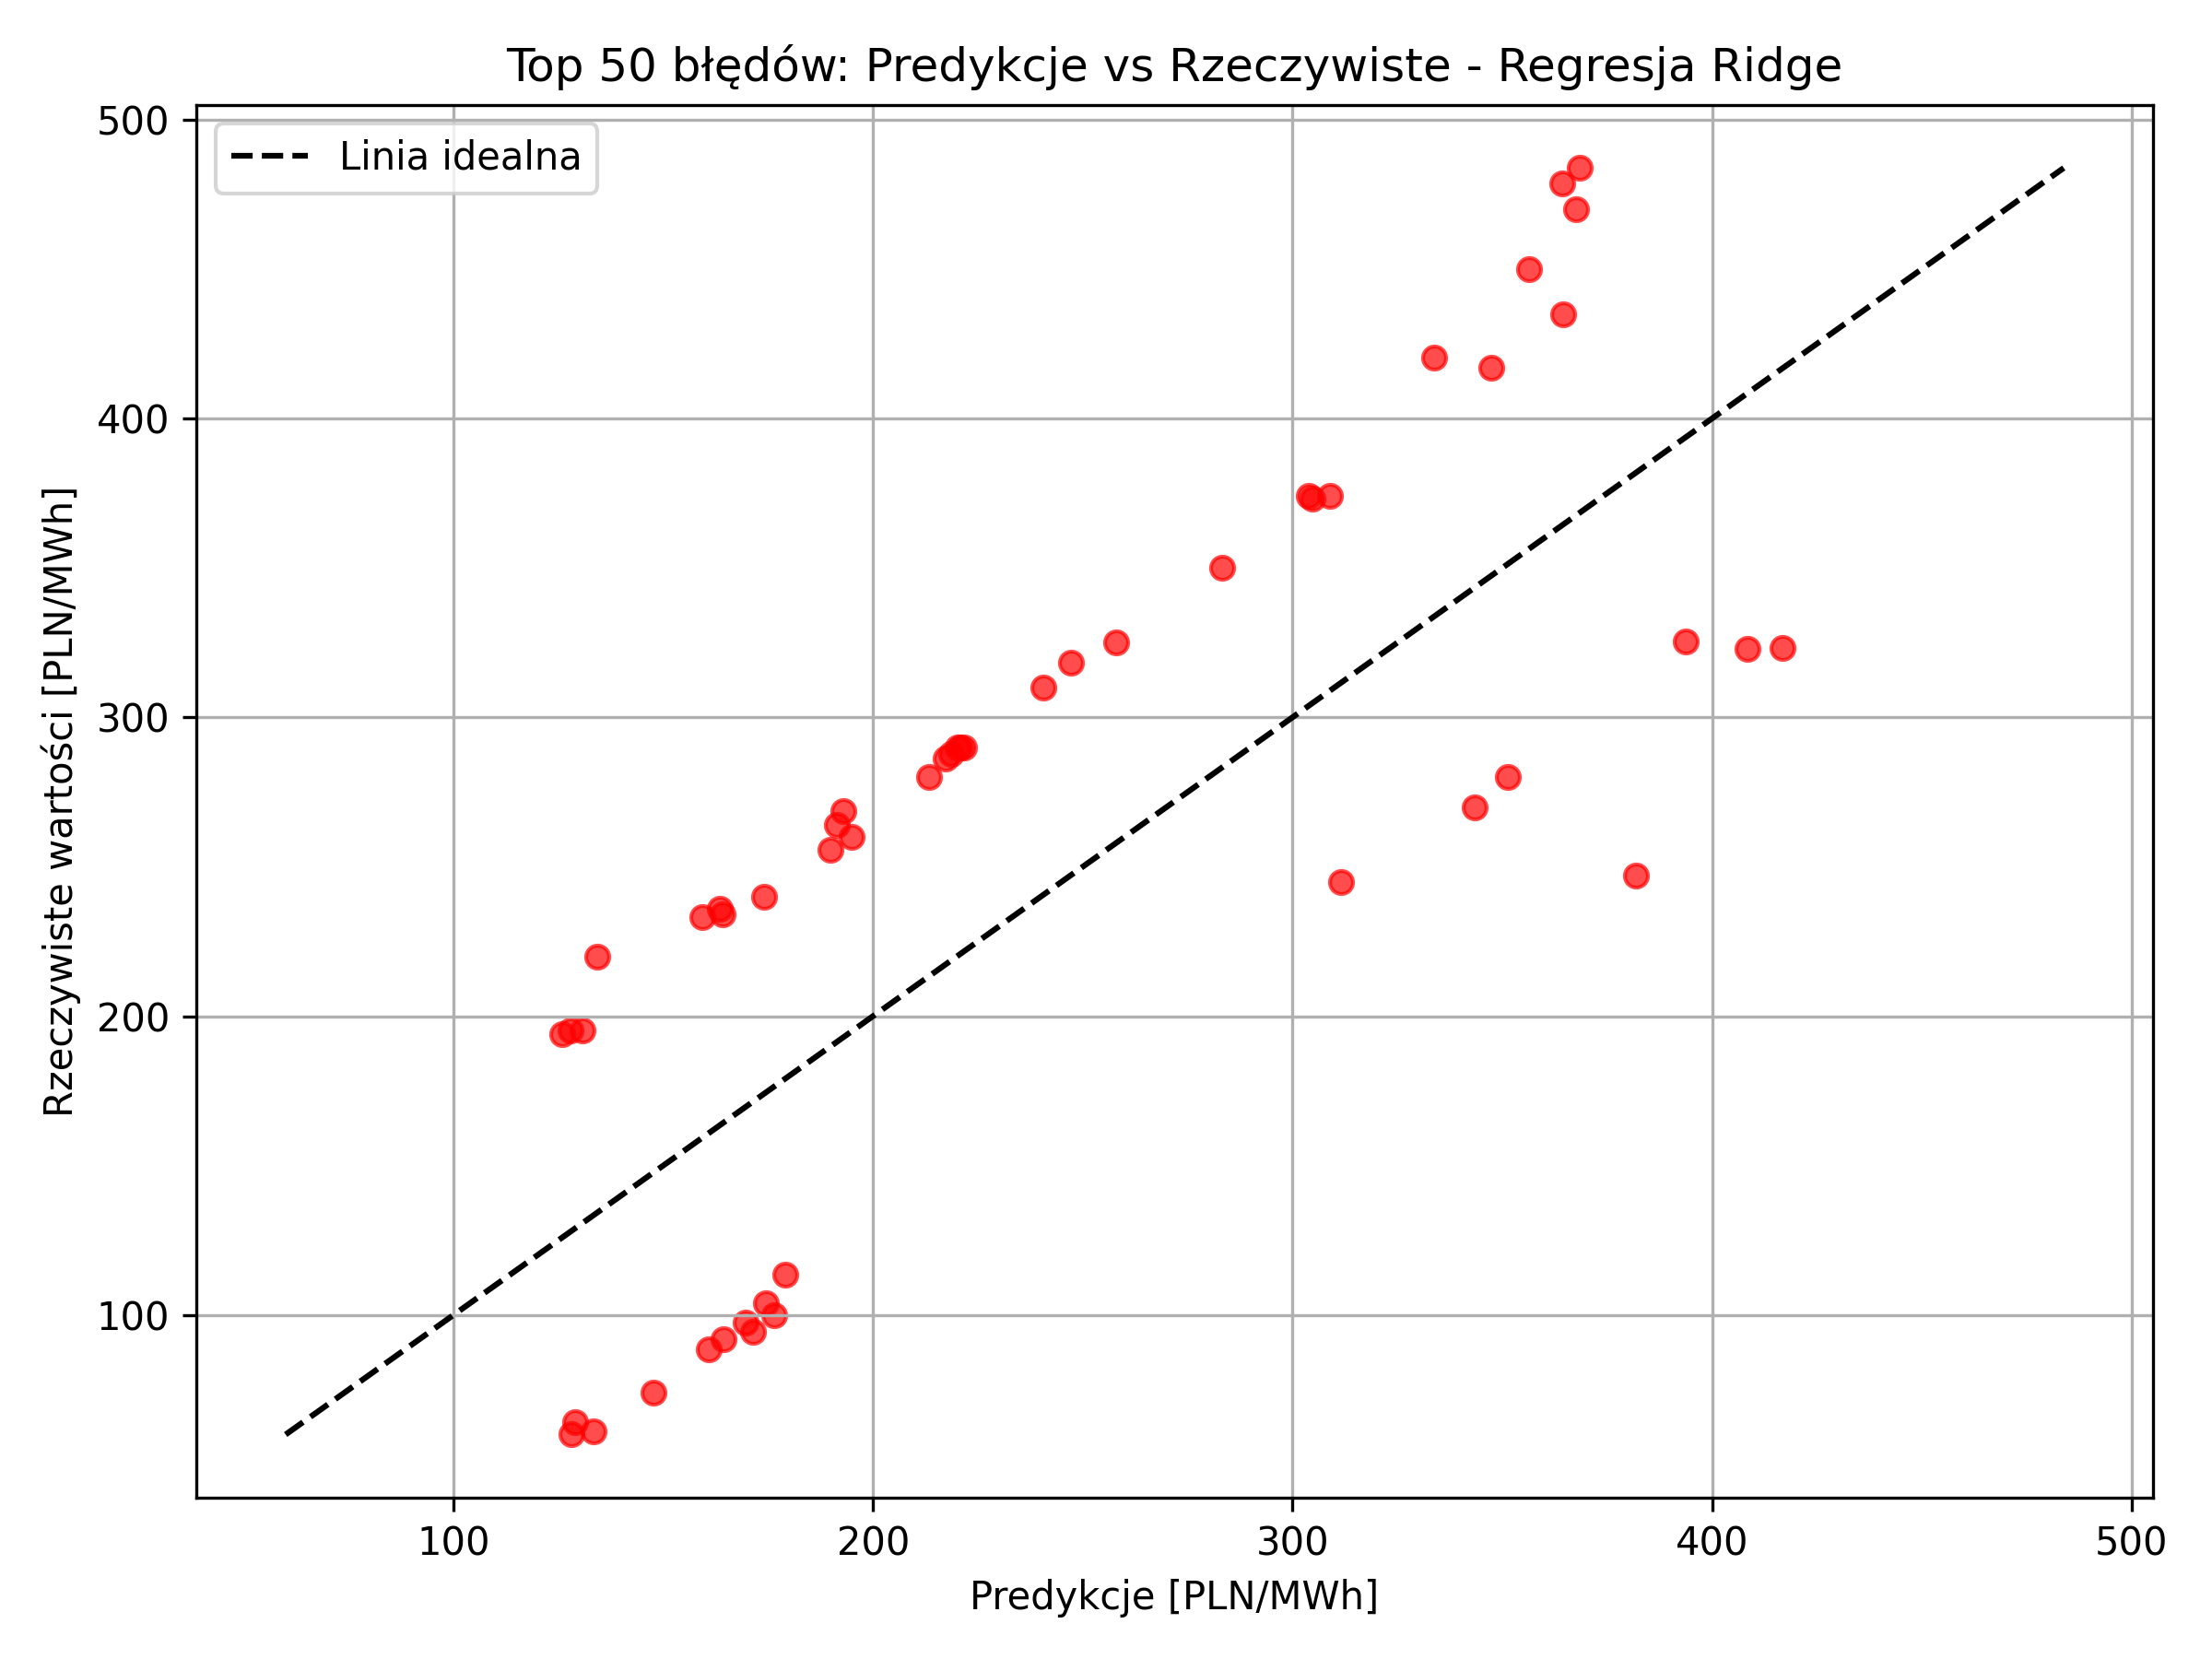
\includegraphics[width=1.0\textwidth]{../../plots/predicts/top_50_errors_Ridge_full_stable_period.png}
    \caption{Największe 50 błędów prognoz dla regresji Ridge w okresie stabilnym. Opracowanie własne.}
    \label{fig:top_50_errors_Ridge_full_stable_period}
\end{figure}

Analiza największych błędów prognoz dla regresji Ridge w okresie stabilnym nie wykazuje istotnych zależności. Wartości błędów nie mają wyraźnych wzorców czasowych ani sezonowych. Pojawienie się dużych błędów wynika z fluktuacji cen energii elektrycznej, wynikających z czynników nie wytłumaczalnych przez zbiór zmiennych objaśniających lub czynników zewnętrzych.

\subsubsection{Prophet}
Model Prophet został skonfigurowany z trybem addytywnym (\texttt{seasonality\_mode='additive'}), ponieważ wstępne testy wykazały, że tryb multiplikatywny (\texttt{seasonality\_mode='multiplicative'}) działa dużo gorzej w przypadku zebranych danych. Tryb multiplikatywny zakłada proporcjonalne skalowanie efektów sezonowych i trendów względem wartości zmiennej objaśnianej, co nie jest odpowiednie dla cen energii elektrycznej, gdzie efekty sezonowe (np. różnice między dniami roboczymi a weekendami) mają raczej charakter addytywny, a nie proporcjonalny.

Testowano różne kombinacje pozostałych hiperparametrów opisanych w rozdziale \ref{subsec:prophet}, aby znaleźć optymalne ustawienia. Najlepsze rezultaty uzyskano dla kombinacji (\texttt{changepoint\_prior\_scale=0.100}, \texttt{seasonality\_prior\_scale=20.0}, \texttt{holidays\_prior\_scale=0.1}), gdzie gdzie MAE wyniosło 15.60, RMSE 20.17, MAPE 7.42\%, a sMAPE 7.33\%. Kombinacja ta charakteryzuje się umiarkowaną elastycznością trendu (\texttt{changepoint\_prior\_scale=0.100}), co pozwala modelowi wychwytywać zmiany w cenach energii (np. stopniowe wzrosty), oraz wysoką elastycznością sezonowości (\texttt{seasonality\_prior\_scale=20.0}), co dobrze oddaje zmienne wzorce dzienne i tygodniowe. Niski wpływ świąt (\texttt{holidays\_prior\_scale=0.1}) sugeruje, że polskie święta mają ograniczony wpływ na ceny energii w tym okresie. Pełne wyniki dla pełnego zbioru danych przedstawiono w tabeli~\ref{tab:prophet_results_combined_stable}.

\begin{table}[H]
    \centering
    \caption{Wyniki modelu Prophet dla pełnego i skróconego zbioru danych w okresie stabilnym (2019).}
    \label{tab:prophet_results_combined_stable}
    \begin{tabular}{|l|cccc|}
        \hline
        \textbf{Zbiór danych} & \textbf{MAE} & \textbf{RMSE} & \textbf{MAPE (\%)} & \textbf{sMAPE (\%)} \\
        \hline
        Pełny     & 15.60 & 20.17 & 7.42 & 7.33 \\
        Skrócony  & 17.75 & 22.85 & 8.17 & 8.32 \\
        \hline
    \end{tabular}
\end{table}

Pełny zbiór danych znowu osiągnął lepsze wyniki od zbioru skróconego. Różnice są większe, niż w przypadku regresji liniowej i Ridge, co sugeruje, że dodatkowe zmienne w pełnym zbiorze danych mają większy wpływ na prognozy modelu Prophet.

Ponizej przedstawiam wykresy rzeczywistych i przewidywanych wartości dla modelu Prophet dla pierwszego kwartału 2019 roku. Wykres jest bardzo podobny do wykresu \ref{fig:ridge_predictions_full_stable_period} dla regresji Ridge.

\begin{figure}[H]
    \centering
    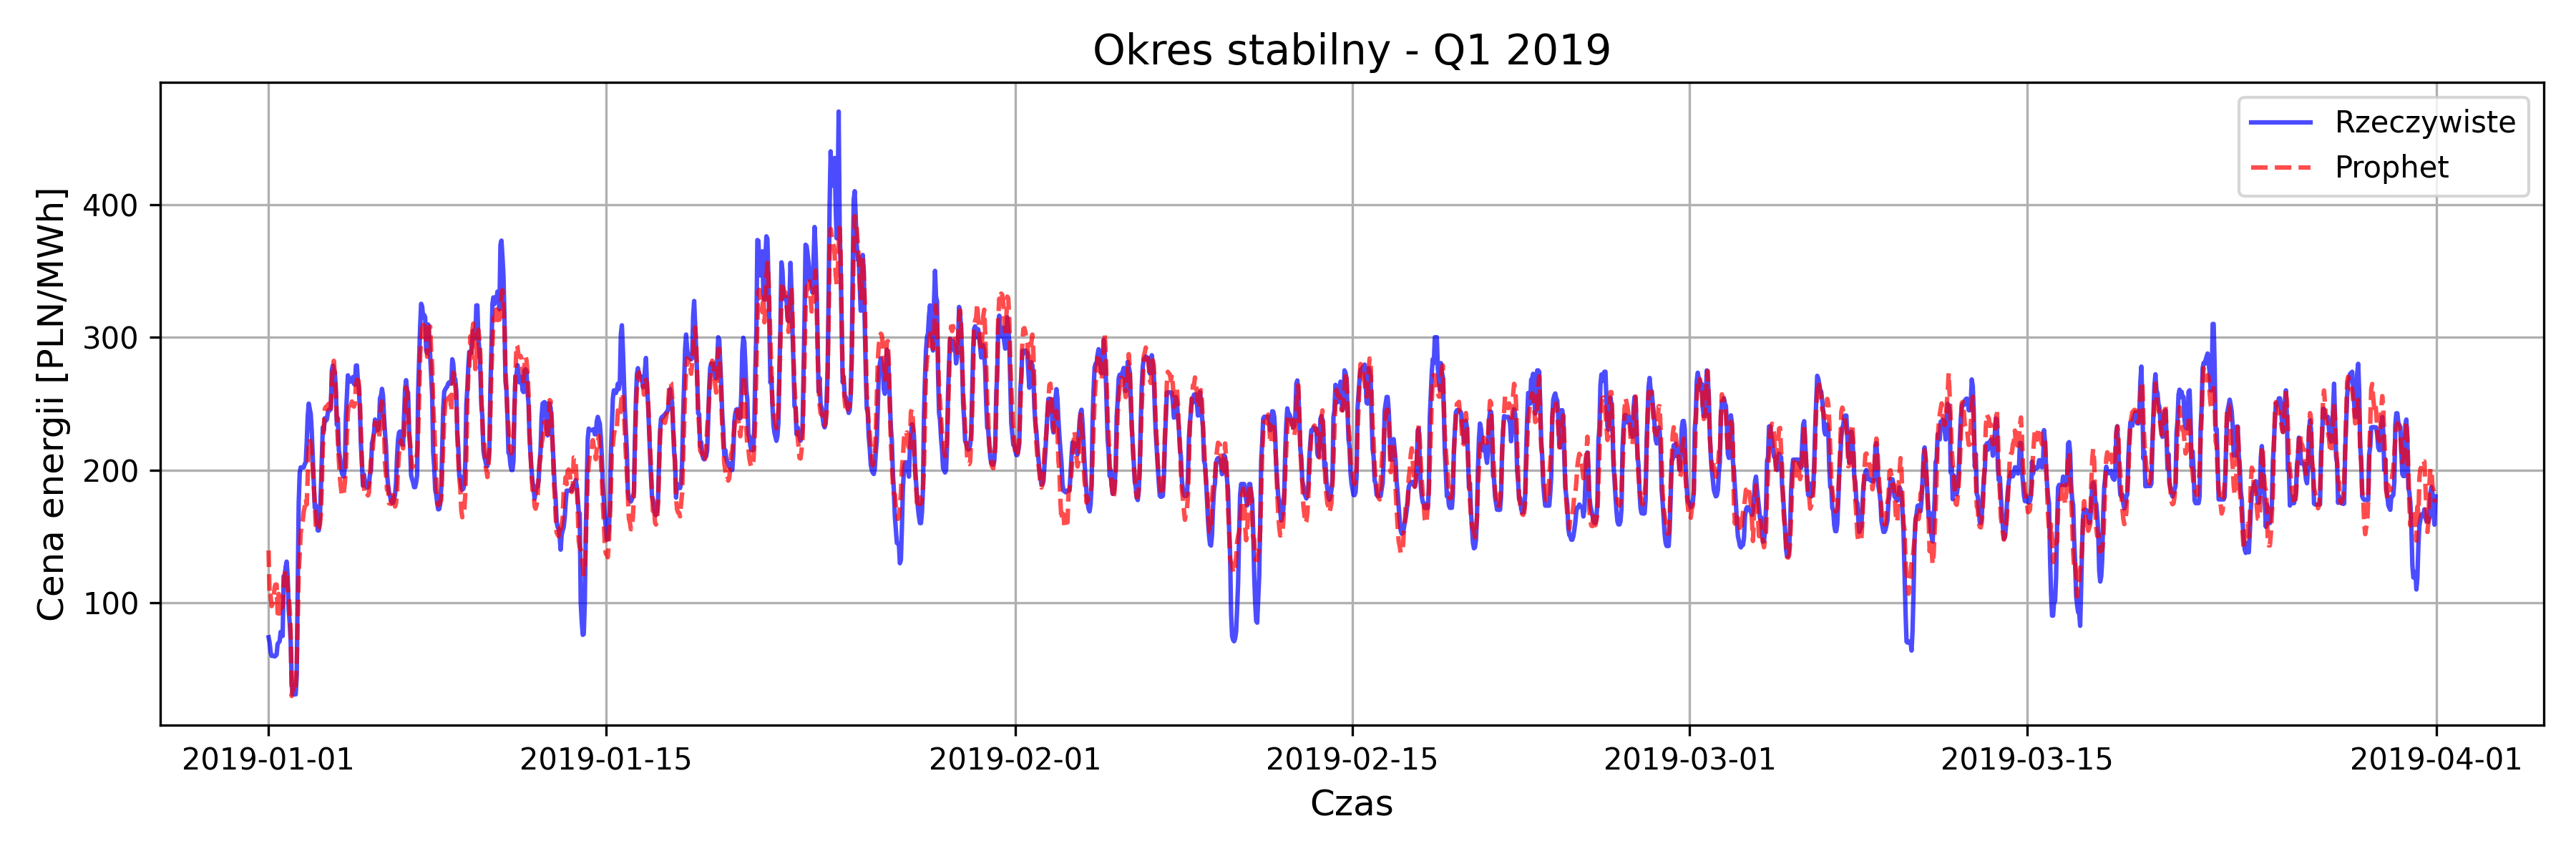
\includegraphics[width=1.0\textwidth]{../../plots/predicts/Prophet_predictions_stable_Q1.png}
    \caption{Porównanie rzeczywistych i przewidywanych wartości cen energii dla modelu Prophet w okresie stabilnym.}
    \label{fig:prophet_predictions_stable_period}
\end{figure}

Wykres jest bardzo podobny do wykresu \ref{fig:ridge_predictions_full_stable_period} dla regresji Ridge. 

Histogram reszt dla modelu Prophet również wykazuje podobieństwo do histogramu reszt dla regresji Ridge~\ref{fig:ridge_residuals_stable_period}. Ma niższy szczyt w okolicy zera, ale agodniejsze zejście w kierunku wartości skrajnych. 

\begin{figure}[H]
    \centering
    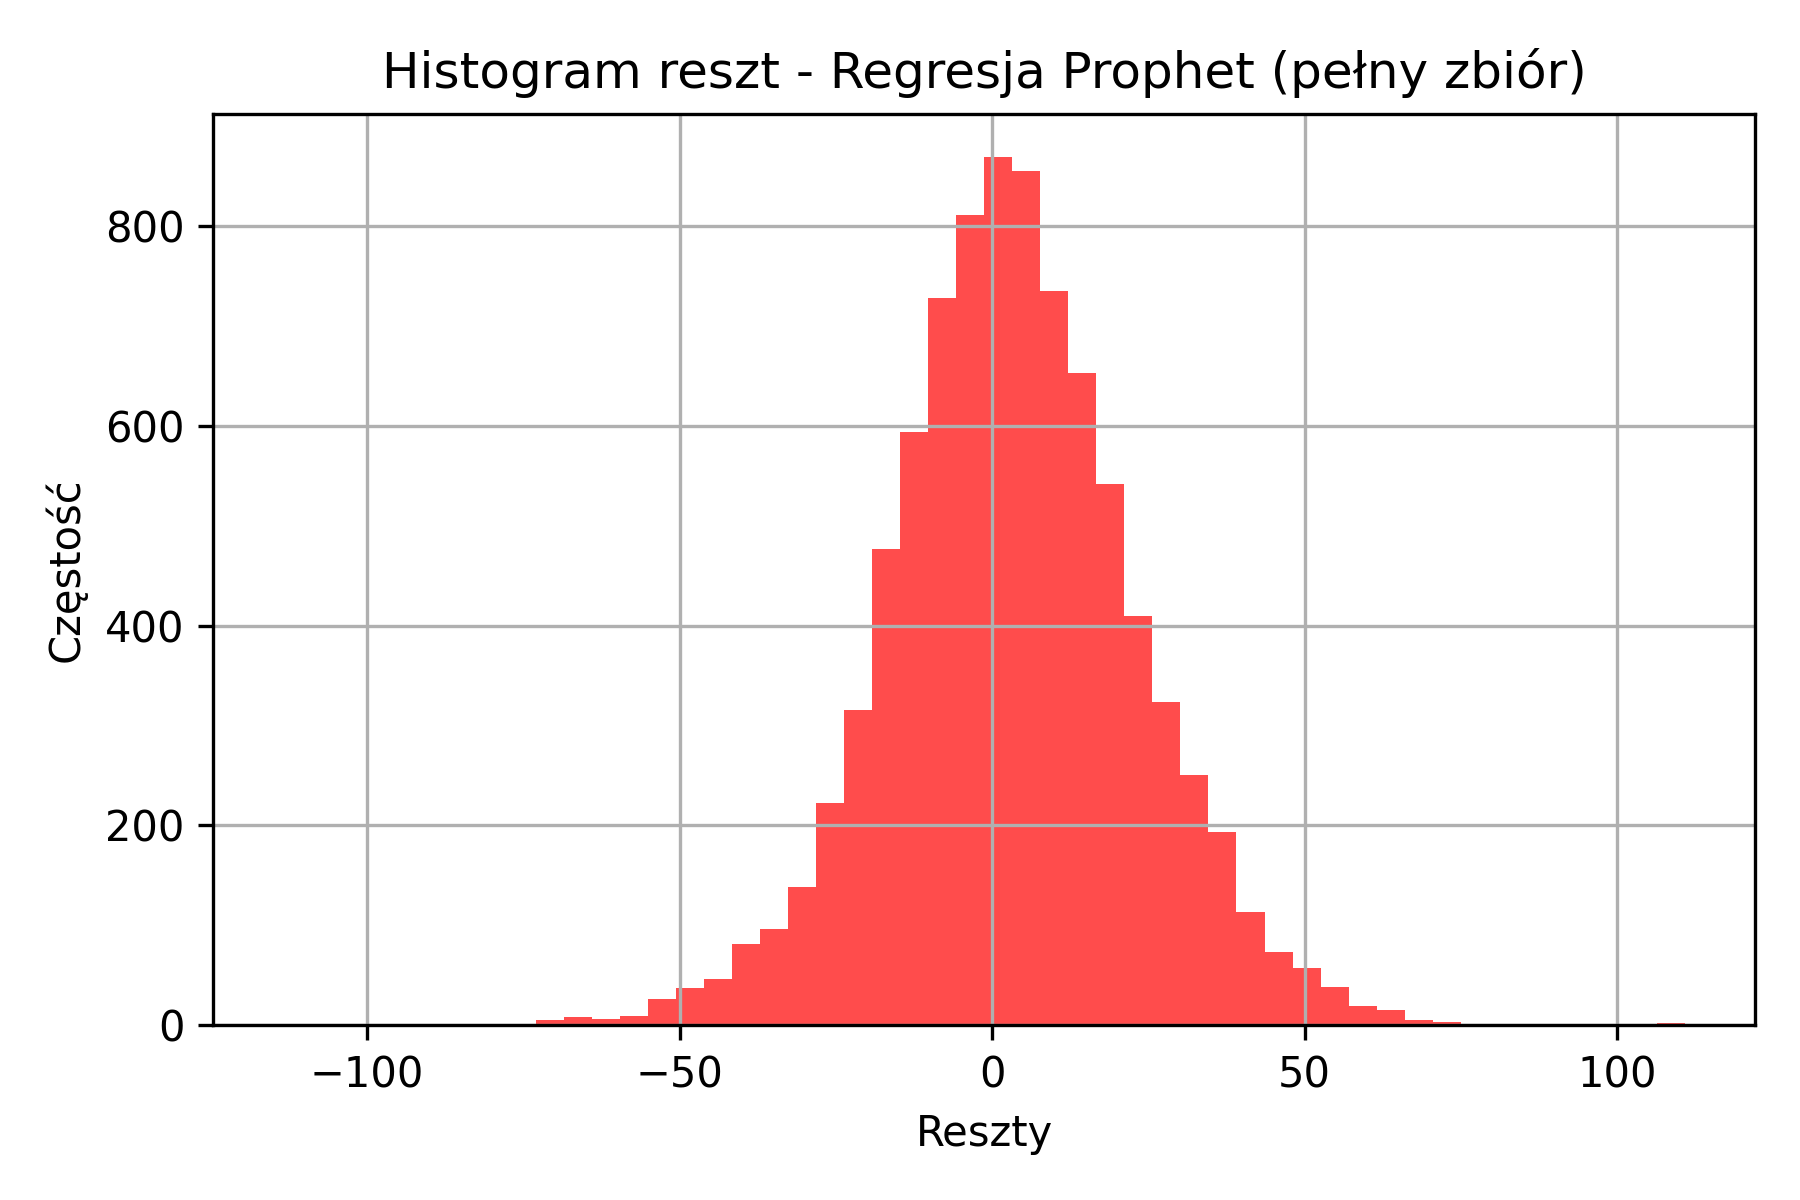
\includegraphics[width=1.0\textwidth]{../../plots/predicts/residuals_histogram_Prophet_full_stable_period_comb_1.png}
    \caption{Histogram reszt dla modelu Prophet w okresie stabilnym.}
    \label{fig:prophet_residuals_stable}
\end{figure}

38 z 50 największych błędów prognoz modelu Prophet występują również w największych błędach prognoz regresji Ridge~\ref{fig:top_50_errors_Ridge_full_stable_period}. Wartości błędów są zbliżone, co sugeruje, że model Prophet uzyskuje podobne wyniki do regresji Ridge. Największym wspólnym błędem prognoz dla obu modeli jest przeszacowanie ceny energii elektrycznej w dniu 10 Marca o godzinie 5 rano, gdzie rzeczywista cena wynosi 64 PLN/MWh, gdzie prognozy wynoszą 129 PLN/MWh oraz 131 PLN/MWh dla modelu Ridge i Prophet. Prawdopodobnie zmienne objaśniające sygnalizują wzrost cen, która nie miała miejsca, co prowadzi do przeszacowania prognoz.

\begin{figure}[H]
    \centering
    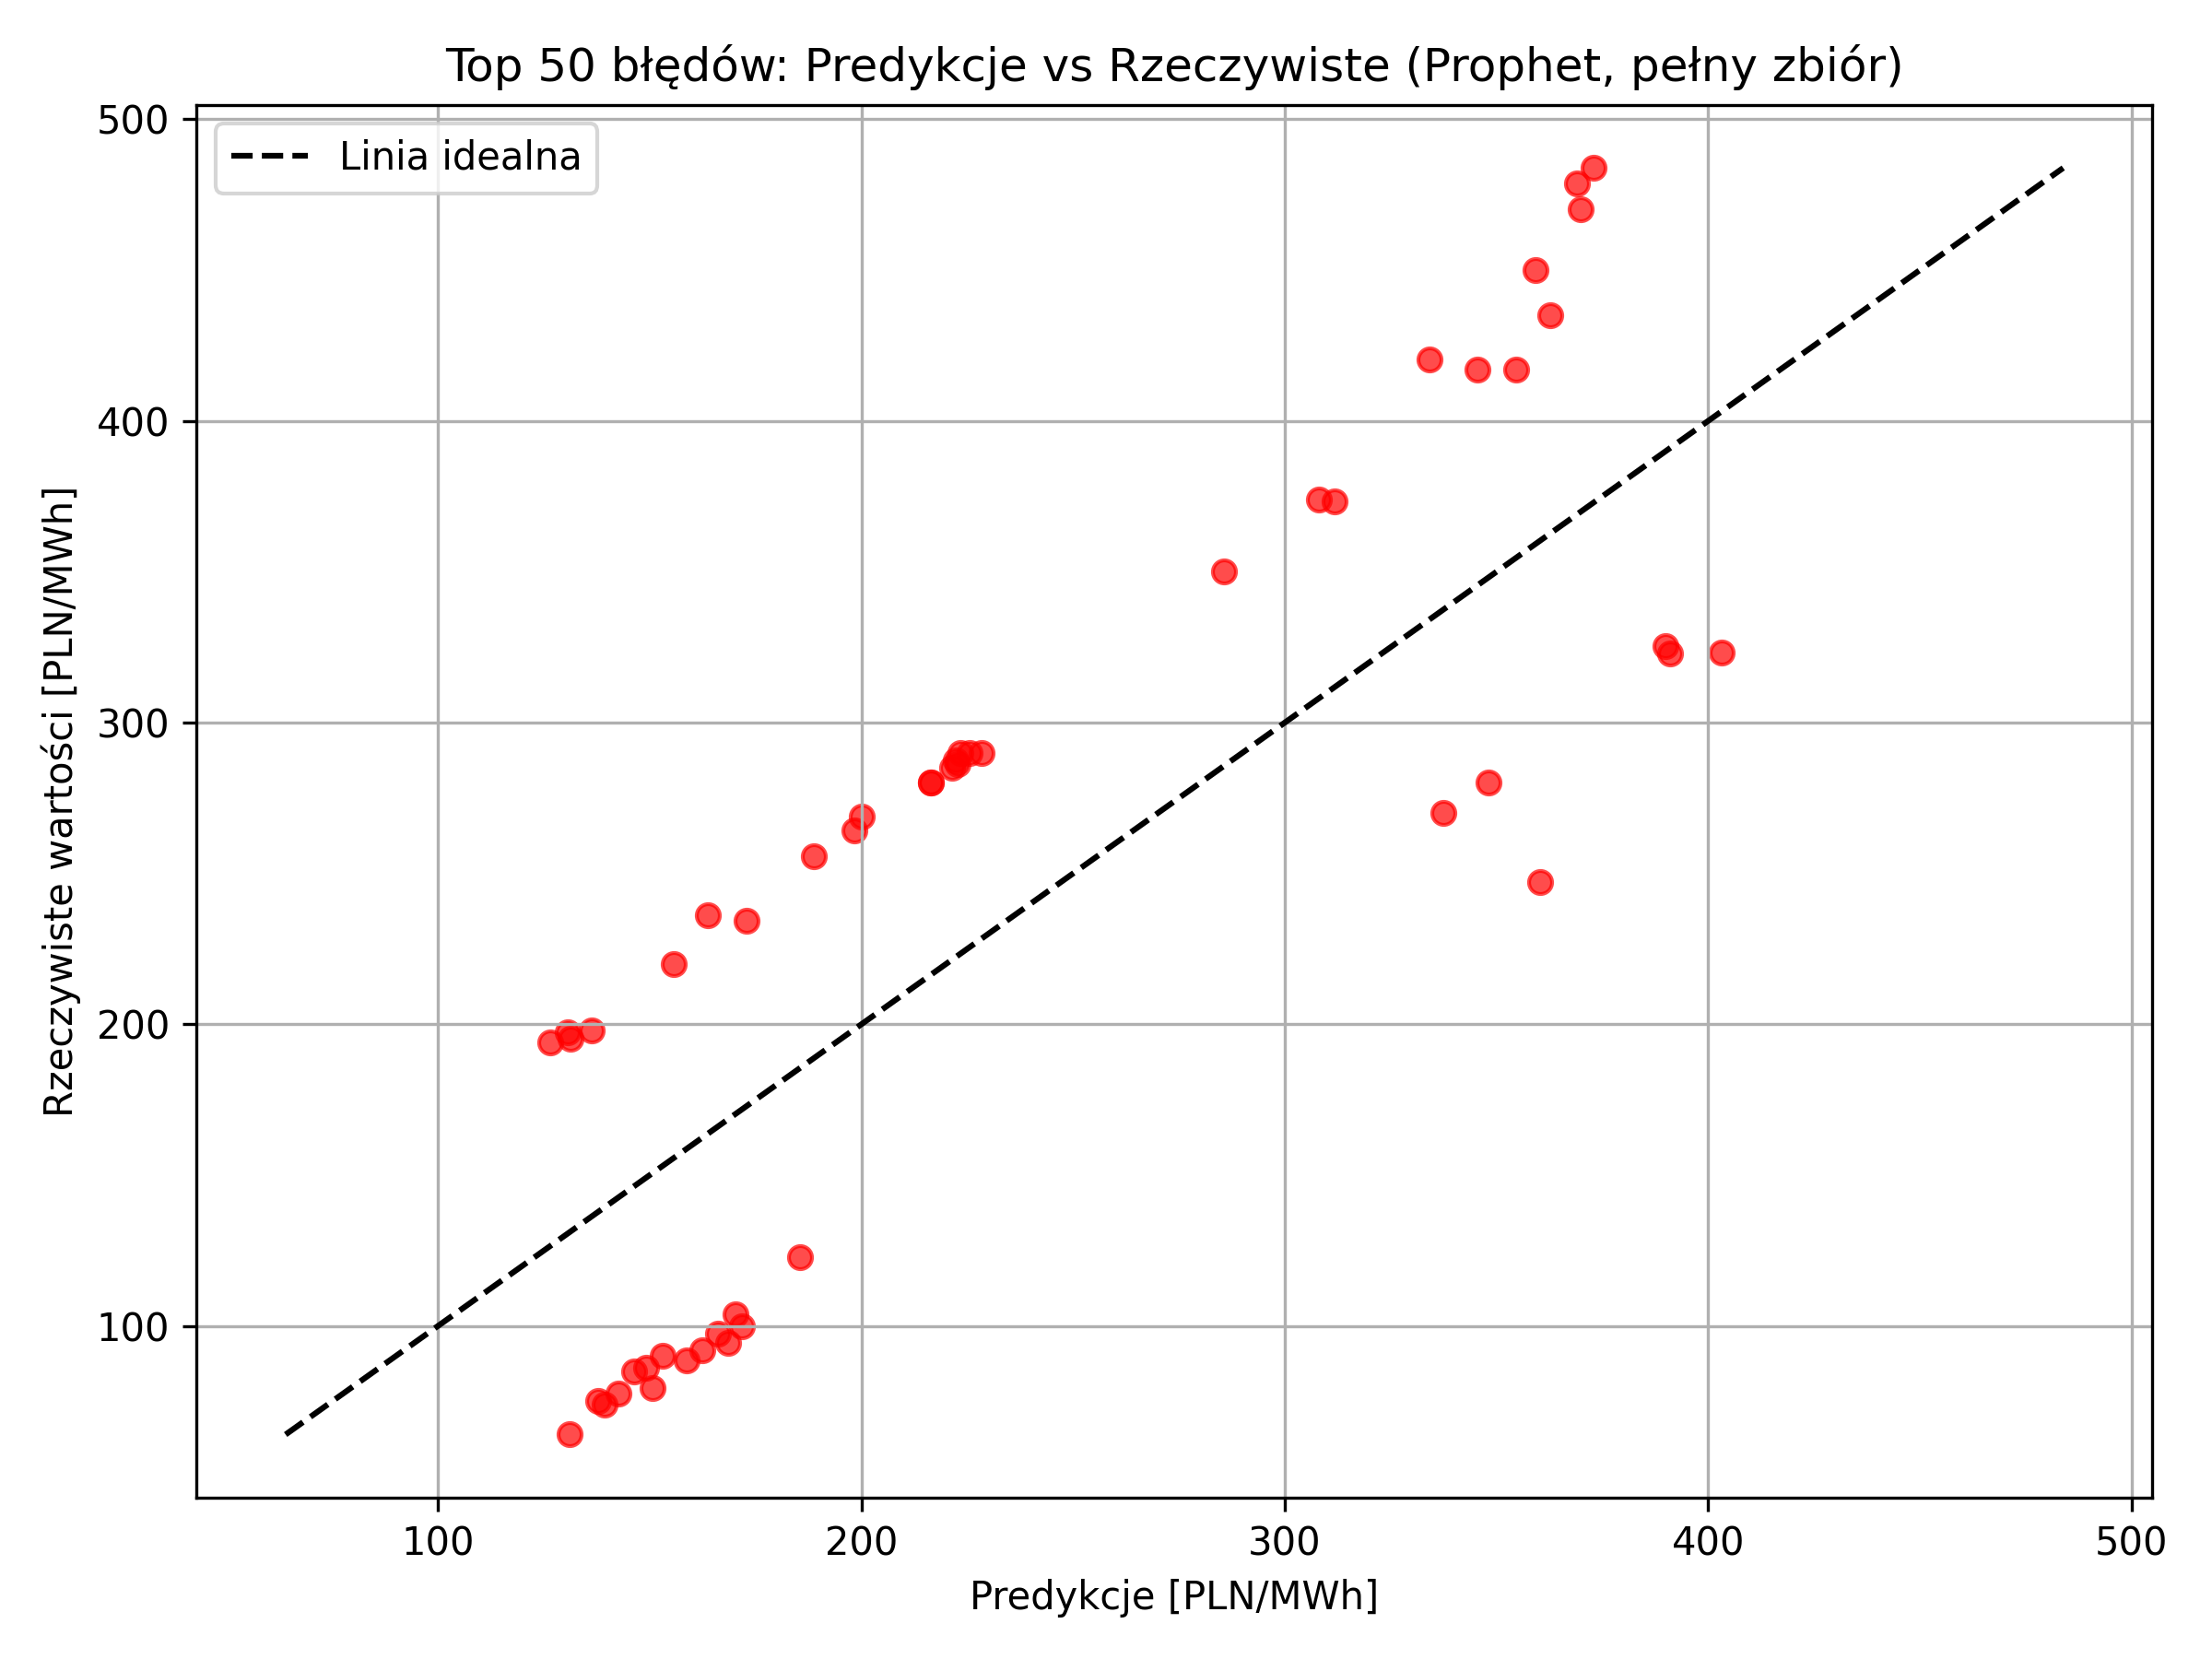
\includegraphics[width=1.0\textwidth]{../../plots/predicts/top_50_errors_Prophet_full_stable_period_comb_1.png}
    \caption{Największe 50 błędów prognoz dla modelu Prophet w okresie stabilnym.}
    \label{fig:top_50_errors_Prophet_stable}
\end{figure}

Analizując wyniki modelu Prophet w odniesieniu do wyników regresji liniowej i grzebietowej, można stwierdzić, że model Prophet osiąga porównywalne wyniki. Wynik MAPE jest o 0.23\% wyższy od regresji Ridge, co sugeruje, że model Prophet nie jest w stanie przewidzieć cen energii elektrycznej lepiej. Natomiast czas wykonania programu w języku programowania \texttt{Python} dla modelu Prophet wynosił ponad 40 sekund, gdzie czas wykonania dla regresji Ridge wynosił 5. W kontekście analizy zebranego zbioru danych, należy zauważyć, że model Prophet nie przynosi żadnych korzyści w porównaniu do regresji Ridge lub liniowej.

\subsubsection{MLP}

Model

\section{Okres niestabilny}
\label{sec:okres_niestabilny}

Okres niestabilny obejmuje lata 2020-2023, w których ceny energii elektrycznej były znacznie bardziej zmienne niż w okresie stabilnym. W związku z tym, okres ten może być bardziej wymagający dla modeli prognozujących.

\subsubsection{Regresja liniowa i Ridge}

W analizie wyników regresji liniowej i Ridge dla okresu niestabilnego (2023) dla pełnego i skróconego zbioru danych obserwuje się zbliżone wartości metryk, co wskazuje na ograniczone różnice w skuteczności obu metod w tym okresie. Tabela~\ref{tab:linear_regression_results} przedstawia szczegółowe wyniki dla regresji liniowej i Ridge. Zbiór skrócony podobnie do okresu stabilnego nie przyniósł znaczących różnic w metrykach, ale dodatkowe zmienne w pełnym zbiorze danych lekko poprawiły wyniki niewielkim kosztem obliczeniowym. 

Wysokie wartości MAPE (powyżej 179\%) sugerują problem z wartościami bliskimi zeru ~\ref{subsec:mape}, które pojawiają się w zbiorze danych z okresu niestabilnego. Z tego powodu, MAPE może nie być najlepszą metryką do oceny skuteczności modeli na zbiorze okresu niestabilnego. Z tego powodu większej uwadze poświęcono metrykom MAE, RMSE, sMAPE oraz \(R^2\). Wartości MAE i RMSE są stosunkowo wysokie, co wskazuje na duże błędy prognozowania w jednostkach absolutncyh. Błąd na poziomie 59.6 PLN/MWh dla MAE oznacza, że prognozy różnią się średnio o 59.6 PLN od rzeczywistych wartości. Może to prowadzić do znacznych strat finansowych, szczególnie w przypadku dużych transakcji. Wartości sMAPE są dwukrotnie wyższe niż w przypadku okresu stabilnego, co sugeruje, że modele mają trudności z przewidywaniem cen energii w okresach dużej zmienności. Pomimo tego, \(R^2\) nie wzrosło znacząco względem okresu stabilnego, co sugeruje, że modele nadal dobrze wyjaśniają zmienność cen energii, mimo dużych błędów prognozowania. 

Najlepsza wartość hiperparametru \(\alpha\) w regresji Ridge dla okresu niestabilnego wyniosła 0.1, co sugeruje, że w tym przypadku współliniowość między zmiennymi objaśniającymi nie jest tak istotna jak w przypadku pełnego zbioru danych w okresie stabilnym. Wartość ta jest znacznie niższa niż w przypadku pełnego zbioru danych w okresie stabilnym (500.0), co może sugerować, że w okresie niestabilnym modele są bardziej elastyczne.

\begin{table}[h]
    \centering
        \caption{Wyniki metryk dla regresji liniowej i Ridge w okresie niestabilnym (2023). Opracowanie własne.}
        \label{tab:linear_regression_results}
        \begin{tabular}{|l|c|c|c|c|c|}
            \hline
            \textbf{Model} & \textbf{MAE} & \textbf{RMSE} & \textbf{MAPE} & \textbf{sMAPE} & \textbf{\(R^2\)} \\
            \hline
            Regresja liniowa (pełny zbiór) & 59.61 & 77.73 & 179.38 & 16.51 & 0.8111 \\
            Regresja liniowa (skrócony zbiór) & 59.76 & 78.07 & 188.24 & 16.68 & 0.8095 \\
            Regresja Ridge (pełny zbiór) & 59.63 & 77.75 & 179.79 & 16.52 & 0.8110 \\
            Regresja Ridge (skrócony zbiór) & 59.78 & 78.08 & 186.22 & 16.69 & 0.8094 \\
            \hline
        \end{tabular}
\end{table}

Wartości metryk są niemal identyczne dla obu modeli, co sugeruje, że w tym przypadku regularyzacja L2 nie przynosi znaczących korzyści.\newline
Dla dobrego zobrazowania prognoz na wykresie wybrano okres o największej zmienności cen w ramach 2023 roku, czyli od 1 września do 31 października. Wartości prognoz dla regresji Ridge w porównaniu do rzeczywistych cen energii elektrycznej przedstawiono na rysunku~\ref{fig:ridge_predictions_full_sep_oct_2023}. Histogram reszt dla modelu Ridge w okresie niestabilnym przedstawiono na rysunku~\ref{fig:residuals_nonstable_histogram_ridge}.

\begin{figure}[H]
    \centering
    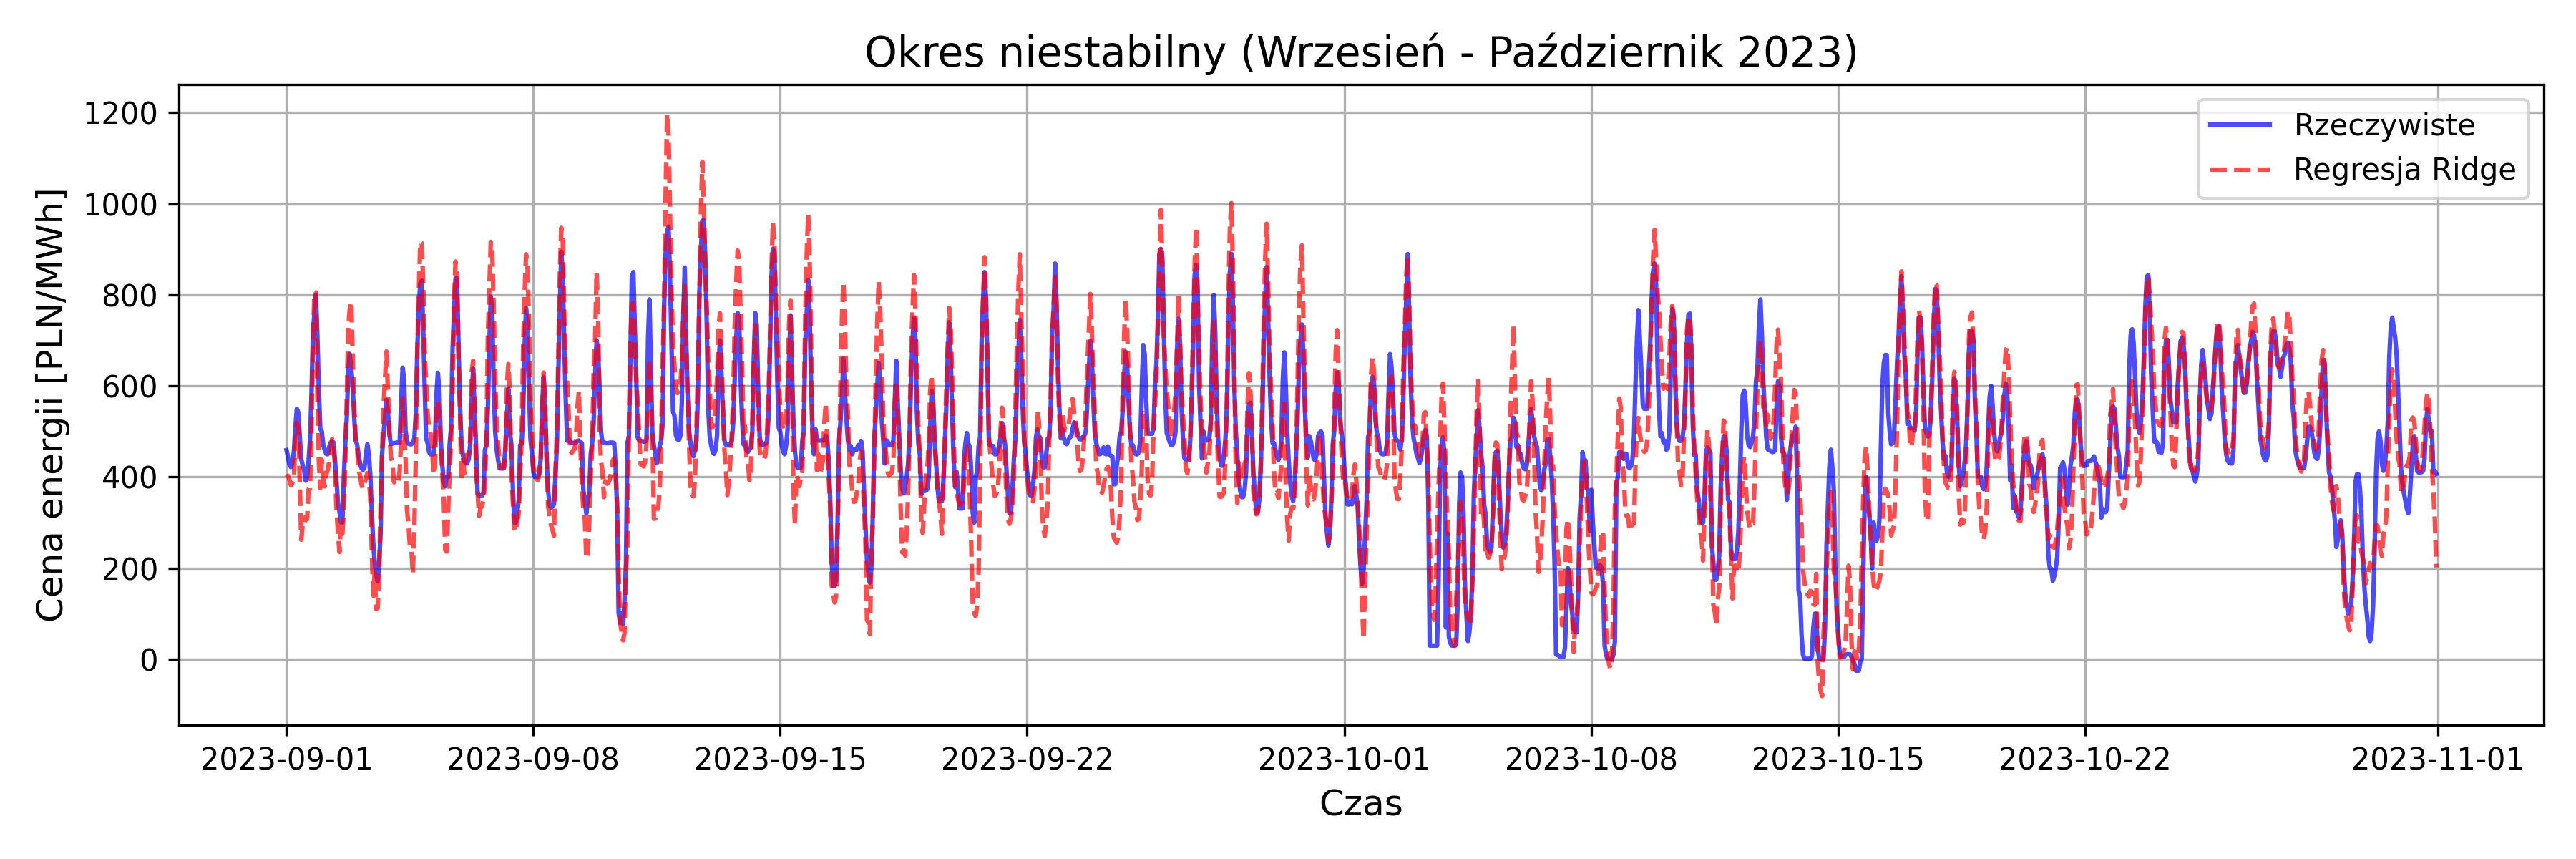
\includegraphics[width=1.0\textwidth]{../../plots/predicts/ridge_predictions_full_sep_oct_2023.png}
    \caption{Prognozy modelu Ridge w porównaniu do rzeczywistych cen energii w okresie niestabilnym (2023).}
    \label{fig:ridge_predictions_full_sep_oct_2023}
\end{figure} 

\begin{figure}[H]
    \centering
    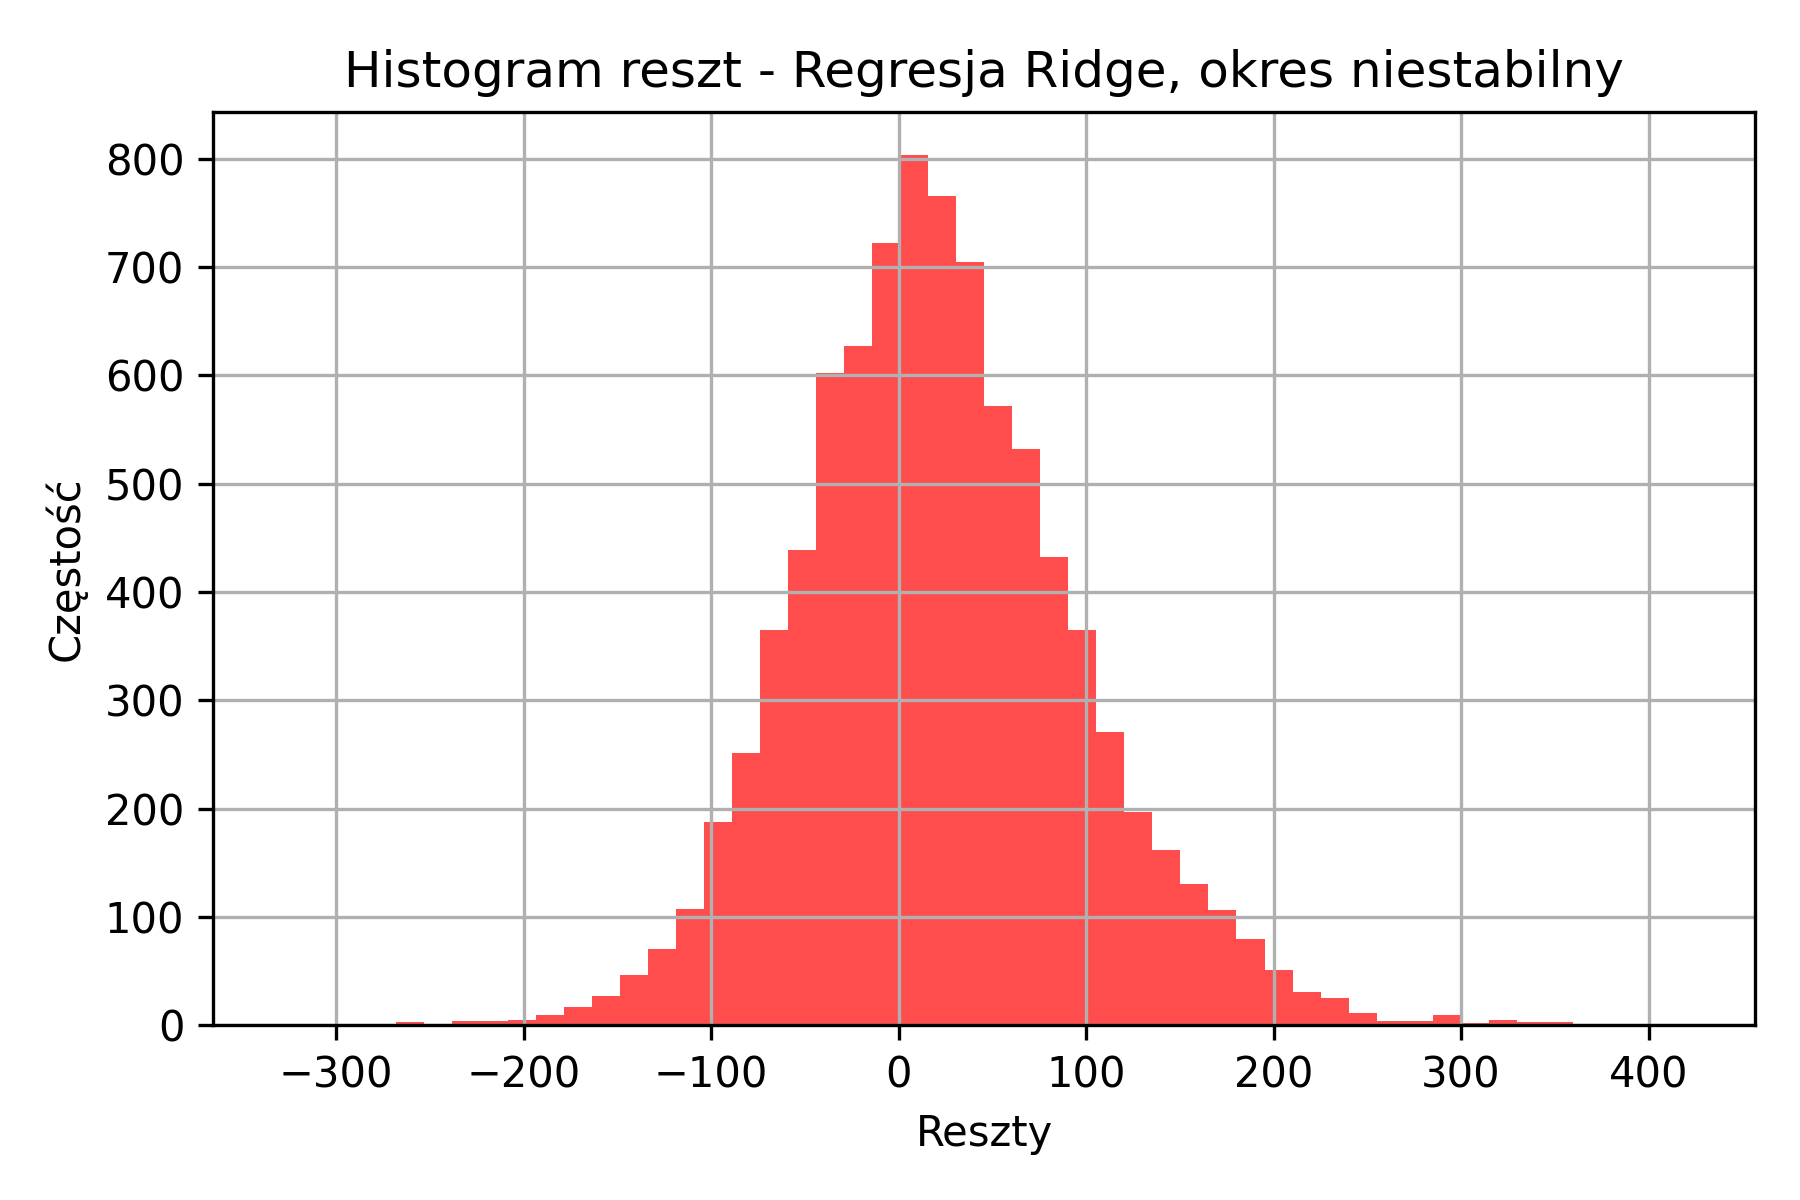
\includegraphics[width=1.0\textwidth]{../../plots/predicts/residuals_histogram_Ridge_not_stable_period.png}
    \caption{Histogram reszt dla modelu Ridge w okresie niestabilnym (2023).}
    \label{fig:residuals_nonstable_histogram_ridge}
\end{figure}

Na podstawie histogramu reszt można zauważyć, że rozkład reszt jest podobny do rozkładu normalnego i ma szczyt w okolicy zera. Porównując histogram reszt z histogramem reszt~\ref{fig:ridge_residuals_stable_period} dla okresu stabilnego, można zauważyć, że histogram reszt w okresie niestabilnym ma szerszy rozkład z większymi ogonami, co potwierdza duże błędy prognozowania w wartościach absolutnych.

Na wykresie największych błędów prognoz dla regresji Ridge w okresie niestabilnym można zauważyć, że największe błędy prognozowania występują powyżej linii odniesienia, co surgeruje, że największe błędy prognozowania są związane z niedooszacowaniem cen energii.

\begin{figure}[H]
    \centering
    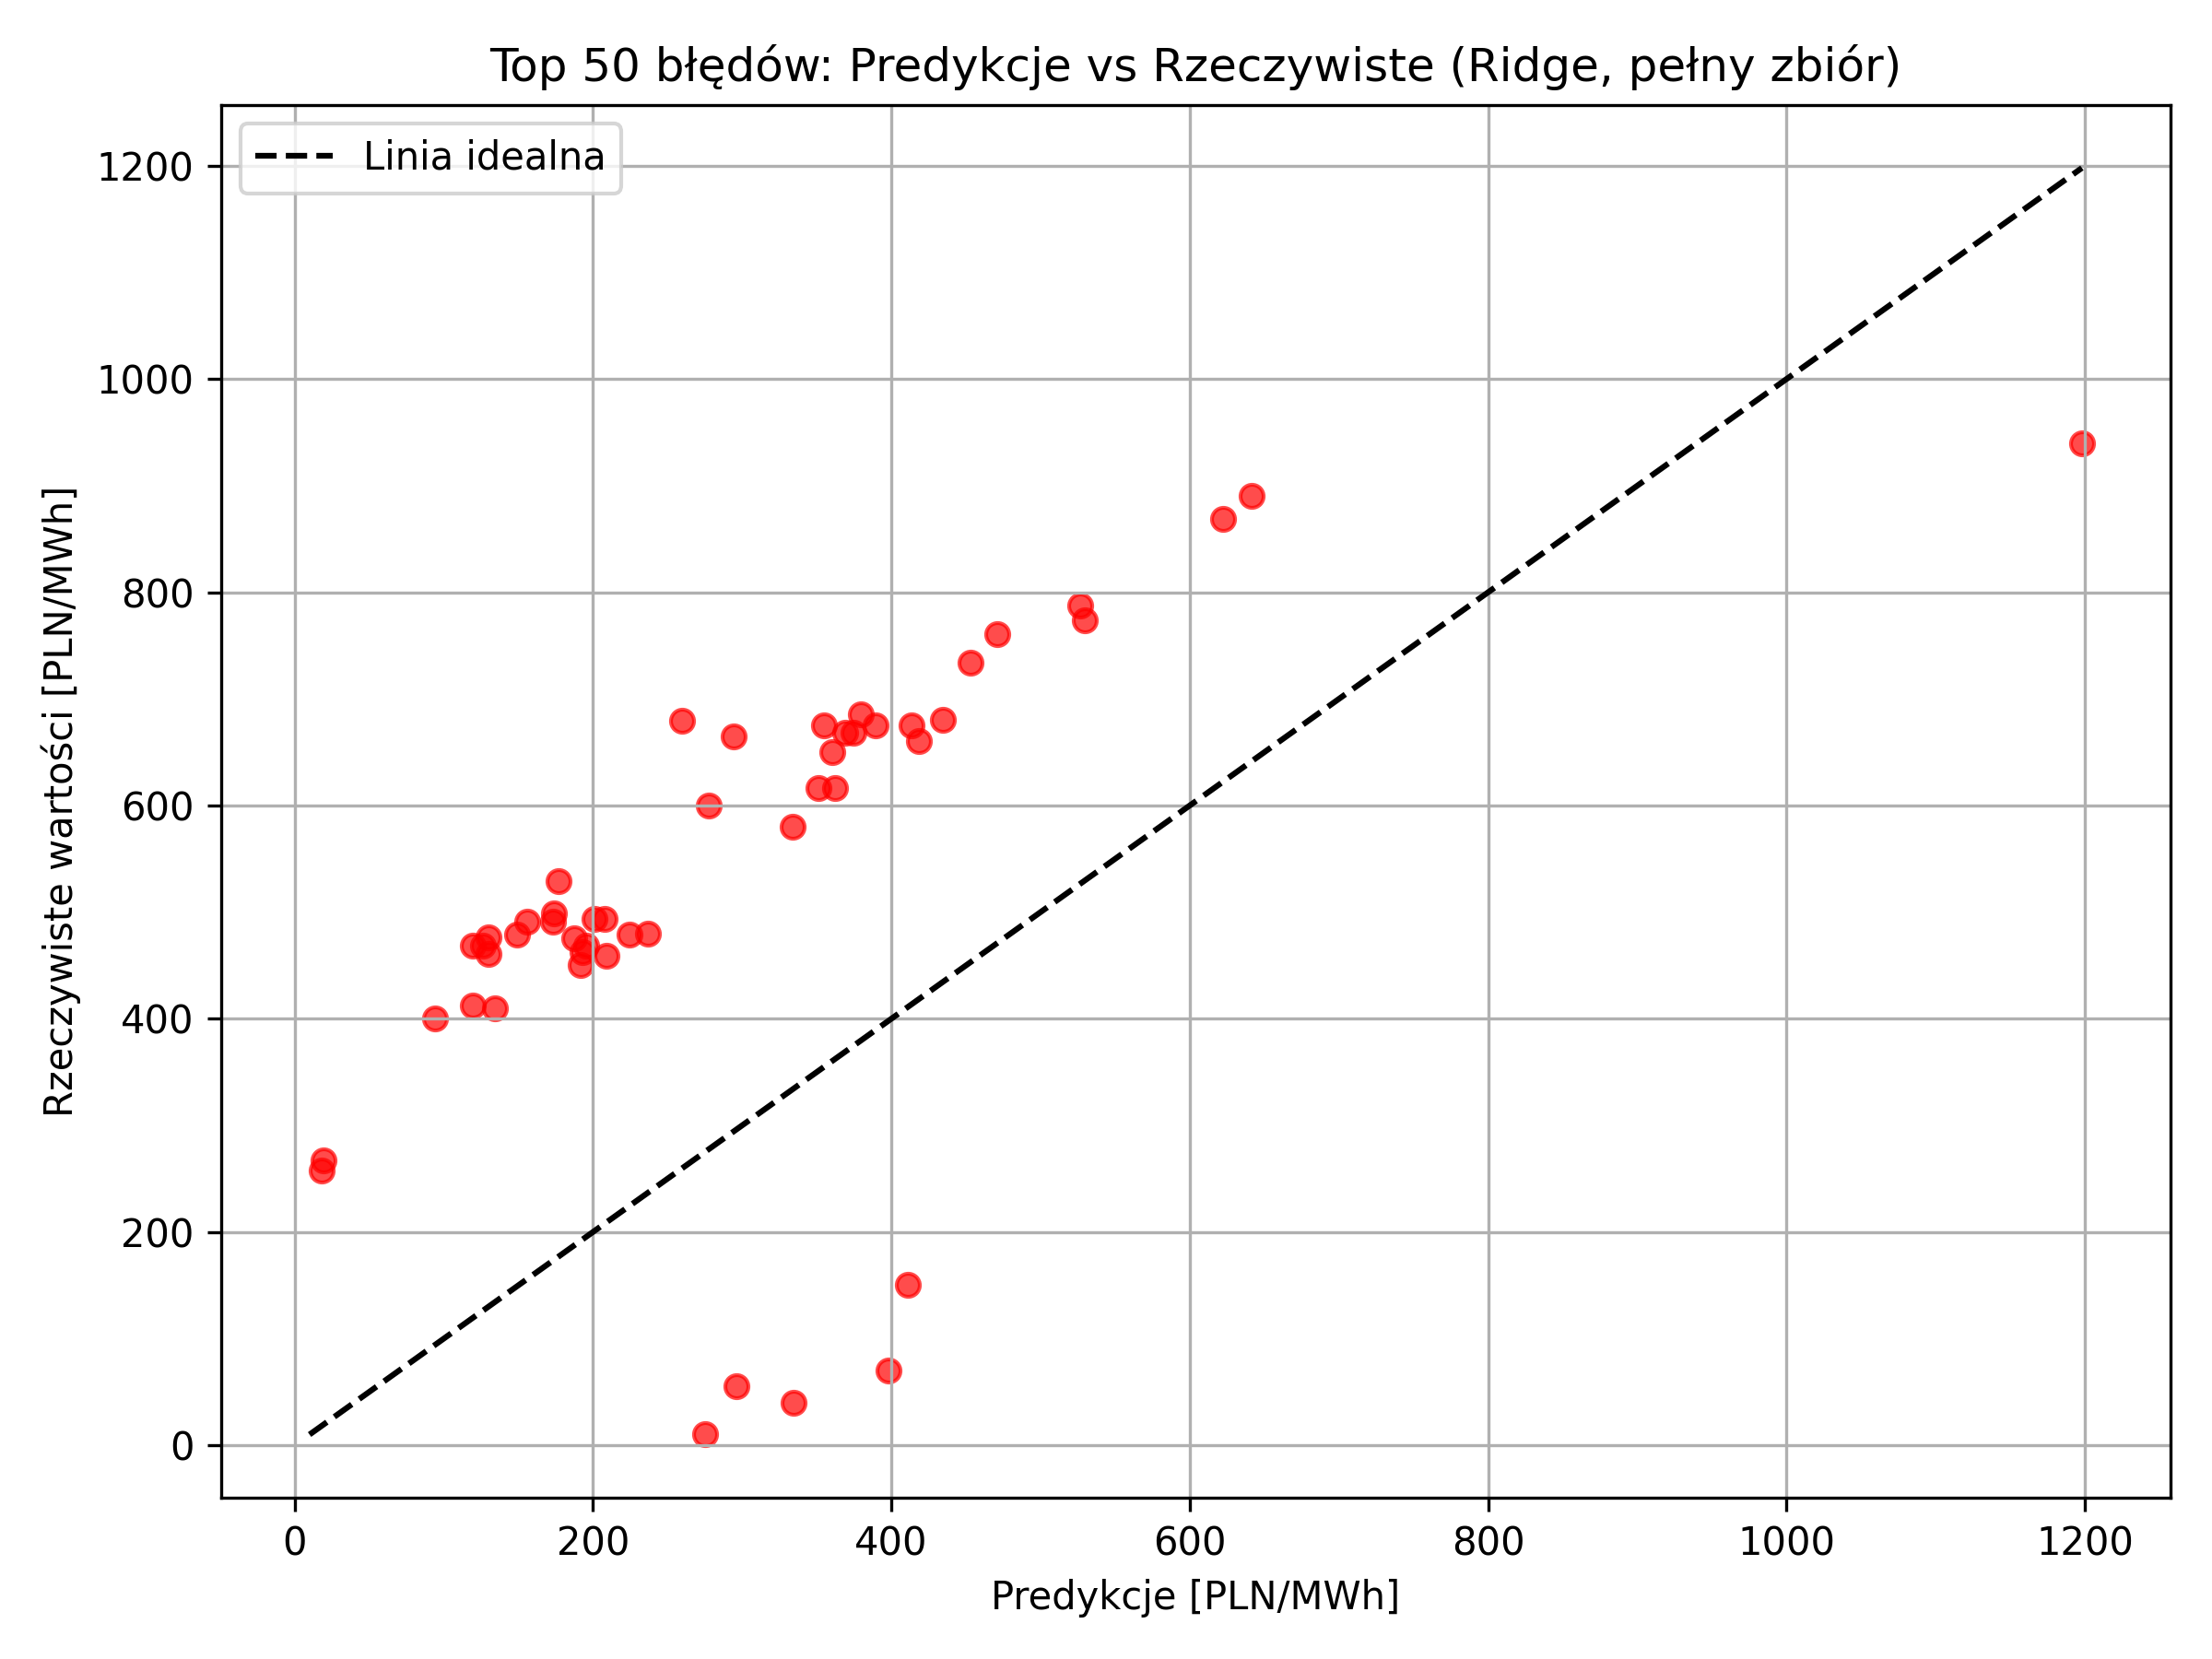
\includegraphics[width=1.0\textwidth]{../../plots/predicts/top_50_errors_Ridge_full_not_stable_period.png}
    \caption{Największe 50 błędów prognoz dla regresji Ridge w okresie niestabilnym (2023).}
    \label{fig:top_50_errors_Ridge_full_not_stable_period}
\end{figure}

\subsubsection{Prophet}

Model Prophet lekko poprawił wyniki w porównaniu do regresji liniowej i Ridge. Najlepszymi parametrami do okresu niestabilnego okazały się (\texttt{changepoint\_prior\_scale=0.001}, \texttt{seasonality\_prior\_scale=50.0}, \texttt{holidays\_prior\_scale=0.1}). Niska wartość {\texttt{changepoint\_prior\_scale}} sugeruje, że model preferuje bardziej stabilne trendy, unikając nadmiernego dopasowania do szumów w danych treningowych. Zwiększona wartość {\texttt{seasonality\_prior\_scale}} pozwala modelowi lepiej uchwycić sezonowe wzorce w danych, co jest istotne w przypadku cen energii elektrycznej, które mogą wykazywać silne sezonowe fluktuacje. Wartość {\texttt{holidays\_prior\_scale}} jest taka sama jak w przypadku okresu stabilnego, co sugeruje, że wpływ świąt na ceny energii wciąż nie jest istotny. Wyniki dla pełnego zbioru danych przedstawiono w tabeli~\ref{tab:prophet_results_combined_nonstable}.

\begin{table}[H]
    \centering
    \caption{Wyniki modelu Prophet dla pełnego i skróconego zbioru danych w okresie niestabilnym (2023).}
    \label{tab:prophet_results_combined_nonstable}
    \begin{tabular}{|l|cccc|}
        \hline
        \textbf{Zbiór danych} & \textbf{MAE} & \textbf{RMSE} & \textbf{MAPE (\%)} & \textbf{sMAPE (\%)} \\
        Pełny     & 57.87 & 74.39 & 163.57 & 16.35 \\
        Skrócony  & 61.10 & 78.56 & 202.72 & 18.17 \\
        \hline
    \end{tabular}
\end{table}

Wartość parametru \texttt{changepoint\_prior\_scale} jest najbardziej znacząca w procesie doboru najlepszych hiperparametrów. Zwiększenie wartości tego parametru do 0.1 prowadzi do znacznego pogorszenia wyników na poziomie \textbf{MAE = 138} oraz \textbf{sMAPE = 20.0\%}. Oznacza to, że model zaczyna być bardziej podatny na wykrywanie zmiany w trendzie i nadmiarowo próbuje dopasować się do lokalnych fluktuacji. Zmiana innych hiperparametrów zwiększa sMAPE o 1\%.

Wynik modelu prophet w porównaniu z regresją Ridge jest nieznacząco lepszy z punktu widzenia sMAPE, ale średni błąd MAE jest o 1.76 PLN/MWh niższy, co może być bardzo istotne z punktu finansowego w przypadku dużych transakcji. Wartości RMSE są również niższe, co sugeruje, że model Prophet lepiej radzi sobie z przewidywaniem cen energii elektrycznej w okresie niestabilnym.

\begin{figure}[H]
    \centering
    \includegraphics[width=1.0\textwidth]{../../plots/predicts/Prophet_predictions_unstable_sep_pełny_comb_1.png}
    \caption{Porównanie rzeczywistych i przewidywanych wartości cen energii dla modelu Prophet w okresie niestabilnym. Opracowanie własne.}
    \label{fig:prophet_predictions_non_stable_period}
\end{figure}

Wykres predykcji modelu Prophet w okresie niestabilnym jest podobny do wykresu regresji Ridge ~\ref{fig:ridge_predictions_full_sep_oct_2023}. Widać, że model przeszacowuje ceny energii elektrycznej w okresach dużej zmienności, co prowadzi do dużych błędów prognozowania. Histogram reszt dla modelu Prophet w okresie niestabilnym przedstawiono na rysunku~\ref{fig:prophet_residuals_non_stable}.

\begin{figure}[H]
    \centering
    \includegraphics[width=1.0\textwidth]{../../plots/predicts/residuals_histogram_Prophet_unstable_pełny_comb_1.png}
    \caption{Histogram reszt dla modelu Prophet w okresie niestabilnym. Opracowanie własne.}
    \label{fig:prophet_residuals_non_stable}
\end{figure}

Histogram posiada nie posaida szczytu w okolicy zera i jest przesunięty w kierunku wartości dodatnich. Ogon histogramu jest również dłuższy w kierunku wartości dodatnich co potwierdza wykres ~\ref{fig:prophet_predictions_non_stable_period}.



\subsubsection{MLP}